\documentclass[twoside]{book}

% Packages required by doxygen
\usepackage{fixltx2e}
\usepackage{calc}
\usepackage{doxygen}
\usepackage[export]{adjustbox} % also loads graphicx
\usepackage{graphicx}
\usepackage[utf8]{inputenc}
\usepackage{makeidx}
\usepackage{multicol}
\usepackage{multirow}
\PassOptionsToPackage{warn}{textcomp}
\usepackage{textcomp}
\usepackage[nointegrals]{wasysym}
\usepackage[table]{xcolor}

% Font selection
\usepackage[T1]{fontenc}
\usepackage[scaled=.90]{helvet}
\usepackage{courier}
\usepackage{amssymb}
\usepackage{sectsty}
\renewcommand{\familydefault}{\sfdefault}
\allsectionsfont{%
  \fontseries{bc}\selectfont%
  \color{darkgray}%
}
\renewcommand{\DoxyLabelFont}{%
  \fontseries{bc}\selectfont%
  \color{darkgray}%
}
\newcommand{\+}{\discretionary{\mbox{\scriptsize$\hookleftarrow$}}{}{}}

% Page & text layout
\usepackage{geometry}
\geometry{%
  a4paper,%
  top=2.5cm,%
  bottom=2.5cm,%
  left=2.5cm,%
  right=2.5cm%
}
\tolerance=750
\hfuzz=15pt
\hbadness=750
\setlength{\emergencystretch}{15pt}
\setlength{\parindent}{0cm}
\setlength{\parskip}{3ex plus 2ex minus 2ex}
\makeatletter
\renewcommand{\paragraph}{%
  \@startsection{paragraph}{4}{0ex}{-1.0ex}{1.0ex}{%
    \normalfont\normalsize\bfseries\SS@parafont%
  }%
}
\renewcommand{\subparagraph}{%
  \@startsection{subparagraph}{5}{0ex}{-1.0ex}{1.0ex}{%
    \normalfont\normalsize\bfseries\SS@subparafont%
  }%
}
\makeatother

% Headers & footers
\usepackage{fancyhdr}
\pagestyle{fancyplain}
\fancyhead[LE]{\fancyplain{}{\bfseries\thepage}}
\fancyhead[CE]{\fancyplain{}{}}
\fancyhead[RE]{\fancyplain{}{\bfseries\leftmark}}
\fancyhead[LO]{\fancyplain{}{\bfseries\rightmark}}
\fancyhead[CO]{\fancyplain{}{}}
\fancyhead[RO]{\fancyplain{}{\bfseries\thepage}}
\fancyfoot[LE]{\fancyplain{}{}}
\fancyfoot[CE]{\fancyplain{}{}}
\fancyfoot[RE]{\fancyplain{}{\bfseries\scriptsize Generated by Doxygen }}
\fancyfoot[LO]{\fancyplain{}{\bfseries\scriptsize Generated by Doxygen }}
\fancyfoot[CO]{\fancyplain{}{}}
\fancyfoot[RO]{\fancyplain{}{}}
\renewcommand{\footrulewidth}{0.4pt}
\renewcommand{\chaptermark}[1]{%
  \markboth{#1}{}%
}
\renewcommand{\sectionmark}[1]{%
  \markright{\thesection\ #1}%
}

% Indices & bibliography
\usepackage{natbib}
\usepackage[titles]{tocloft}
\setcounter{tocdepth}{3}
\setcounter{secnumdepth}{5}
\makeindex

% Hyperlinks (required, but should be loaded last)
\usepackage{ifpdf}
\ifpdf
  \usepackage[pdftex,pagebackref=true]{hyperref}
\else
  \usepackage[ps2pdf,pagebackref=true]{hyperref}
\fi
\hypersetup{%
  colorlinks=true,%
  linkcolor=blue,%
  citecolor=blue,%
  unicode%
}

% Custom commands
\newcommand{\clearemptydoublepage}{%
  \newpage{\pagestyle{empty}\cleardoublepage}%
}

\usepackage{caption}
\captionsetup{labelsep=space,justification=centering,font={bf},singlelinecheck=off,skip=4pt,position=top}

%===== C O N T E N T S =====

\begin{document}

% Titlepage & ToC
\hypersetup{pageanchor=false,
             bookmarksnumbered=true,
             pdfencoding=unicode
            }
\pagenumbering{alph}
\begin{titlepage}
\vspace*{7cm}
\begin{center}%
{\Large MA Dissertation \\[1ex]\large 1 }\\
\vspace*{1cm}
{\large Generated by Doxygen 1.8.14}\\
\end{center}
\end{titlepage}
\clearemptydoublepage
\pagenumbering{roman}
\tableofcontents
\clearemptydoublepage
\pagenumbering{arabic}
\hypersetup{pageanchor=true}

%--- Begin generated contents ---
\chapter{Hierarchical Index}
\section{Class Hierarchy}
This inheritance list is sorted roughly, but not completely, alphabetically\+:\begin{DoxyCompactList}
\item \contentsline{section}{All\+Overall\+Player\+Data}{\pageref{struct_all_overall_player_data}}{}
\item \contentsline{section}{Level\+Generation.\+Averages}{\pageref{struct_level_generation_1_1_averages}}{}
\item \contentsline{section}{Character\+Start\+Data}{\pageref{struct_character_start_data}}{}
\item \contentsline{section}{Level\+Generation.\+Data\+Averages}{\pageref{struct_level_generation_1_1_data_averages}}{}
\item \contentsline{section}{Design\+Data}{\pageref{class_design_data}}{}
\item \contentsline{section}{Input\+Scheme\+Objects}{\pageref{struct_input_scheme_objects}}{}
\item \contentsline{section}{Level\+Data}{\pageref{class_level_data}}{}
\item Mono\+Behaviour\begin{DoxyCompactList}
\item \contentsline{section}{About}{\pageref{class_about}}{}
\item \contentsline{section}{Camera\+Movement}{\pageref{class_camera_movement}}{}
\item \contentsline{section}{Canvas\+Manager}{\pageref{class_canvas_manager}}{}
\item \contentsline{section}{Character}{\pageref{class_character}}{}
\begin{DoxyCompactList}
\item \contentsline{section}{Player}{\pageref{class_player}}{}
\end{DoxyCompactList}
\item \contentsline{section}{Collectable}{\pageref{class_collectable}}{}
\item \contentsline{section}{Control\+Scheme}{\pageref{class_control_scheme}}{}
\item \contentsline{section}{End\+Zone}{\pageref{class_end_zone}}{}
\item \contentsline{section}{Enemy}{\pageref{class_enemy}}{}
\item \contentsline{section}{Game\+Canvas}{\pageref{class_game_canvas}}{}
\item \contentsline{section}{Grinder\+Obstacle}{\pageref{class_grinder_obstacle}}{}
\item \contentsline{section}{Level\+Generation.\+Grid}{\pageref{class_level_generation_1_1_grid}}{}
\item \contentsline{section}{Level\+Generation.\+Level\+Generator}{\pageref{class_level_generation_1_1_level_generator}}{}
\item \contentsline{section}{Level\+Generation.\+Room}{\pageref{class_level_generation_1_1_room}}{}
\item \contentsline{section}{Main\+Menu}{\pageref{class_main_menu}}{}
\item \contentsline{section}{One\+Way\+Platform}{\pageref{class_one_way_platform}}{}
\item \contentsline{section}{Pathing\+Object}{\pageref{class_pathing_object}}{}
\item \contentsline{section}{Room\+Exit}{\pageref{class_room_exit}}{}
\item \contentsline{section}{Screenshot}{\pageref{class_screenshot}}{}
\item \contentsline{section}{Utilities.\+Singleton$<$ T $>$}{\pageref{class_utilities_1_1_singleton}}{}
\end{DoxyCompactList}
\item \contentsline{section}{Overall\+Player\+Data}{\pageref{struct_overall_player_data}}{}
\item \contentsline{section}{Player\+Data}{\pageref{struct_player_data}}{}
\item \contentsline{section}{Playthrough\+Data}{\pageref{class_playthrough_data}}{}
\item \contentsline{section}{Scene\+Data}{\pageref{struct_scene_data}}{}
\item Scriptable\+Object\begin{DoxyCompactList}
\item \contentsline{section}{Base\+Averages}{\pageref{class_base_averages}}{}
\item \contentsline{section}{Level\+Generation.\+Template\+Holder}{\pageref{class_level_generation_1_1_template_holder}}{}
\end{DoxyCompactList}
\item \contentsline{section}{Simple\+Room\+Data}{\pageref{struct_simple_room_data}}{}
\item \contentsline{section}{Utilities.\+Singleton$<$ Database\+Manager $>$}{\pageref{class_utilities_1_1_singleton}}{}
\begin{DoxyCompactList}
\item \contentsline{section}{Database\+Manager}{\pageref{class_database_manager}}{}
\end{DoxyCompactList}
\item \contentsline{section}{Utilities.\+Singleton$<$ Data\+Tracker $>$}{\pageref{class_utilities_1_1_singleton}}{}
\begin{DoxyCompactList}
\item \contentsline{section}{Data\+Tracker}{\pageref{class_data_tracker}}{}
\end{DoxyCompactList}
\item \contentsline{section}{Utilities.\+Singleton$<$ Game\+Manager $>$}{\pageref{class_utilities_1_1_singleton}}{}
\begin{DoxyCompactList}
\item \contentsline{section}{Game\+Manager}{\pageref{class_game_manager}}{}
\end{DoxyCompactList}
\item \contentsline{section}{Utilities.\+Singleton$<$ Scene\+Loader $>$}{\pageref{class_utilities_1_1_singleton}}{}
\begin{DoxyCompactList}
\item \contentsline{section}{Scene\+Loader}{\pageref{class_scene_loader}}{}
\end{DoxyCompactList}
\item \contentsline{section}{Level\+Generation.\+Template\+Group}{\pageref{class_level_generation_1_1_template_group}}{}
\end{DoxyCompactList}

\chapter{Class Index}
\section{Class List}
Here are the classes, structs, unions and interfaces with brief descriptions\+:\begin{DoxyCompactList}
\item\contentsline{section}{\mbox{\hyperlink{class_game_manager}{Game\+Manager}} \\*Manages game and its states }{\pageref{class_game_manager}}{}
\end{DoxyCompactList}

\chapter{File Index}
\section{File List}
Here is a list of all files with brief descriptions\+:\begin{DoxyCompactList}
\item\contentsline{section}{C\+:/\+Users/louca/\+Documents/\+M\+A\+Dissertation/\+M\+A\+Dissertation/\+M\+A\+Dissertation/\+Assets/\+Classes/\mbox{\hyperlink{_game_manager_8cs}{Game\+Manager.\+cs}} }{\pageref{_game_manager_8cs}}{}
\end{DoxyCompactList}

\chapter{Class Documentation}
\hypertarget{class_game_manager}{}\section{Game\+Manager Class Reference}
\label{class_game_manager}\index{Game\+Manager@{Game\+Manager}}


Manages game and its states  


Inheritance diagram for Game\+Manager\+:\begin{figure}[H]
\begin{center}
\leavevmode
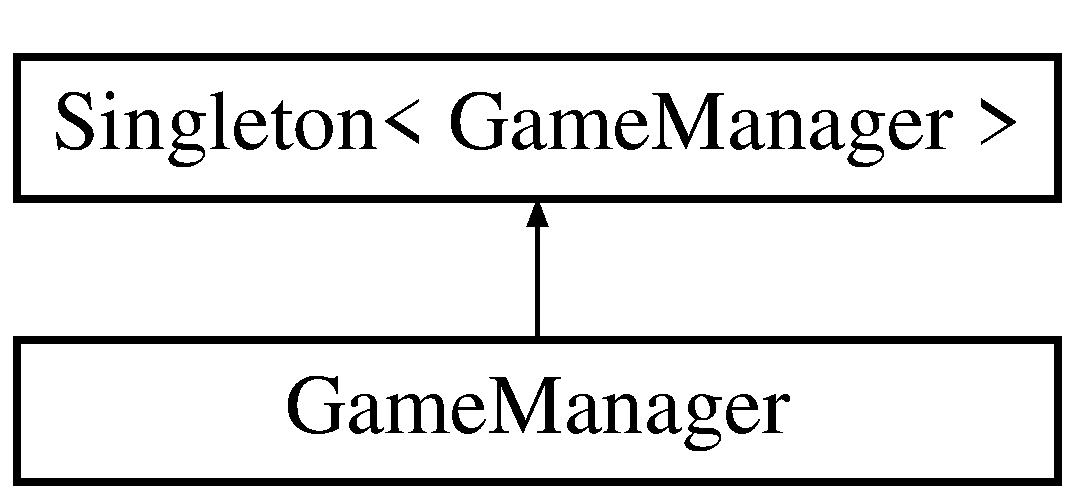
\includegraphics[height=2.000000cm]{class_game_manager}
\end{center}
\end{figure}
\subsection*{Public Member Functions}
\begin{DoxyCompactItemize}
\item 
void \mbox{\hyperlink{class_game_manager_a38cc549d56890d3d3097e0a81fd7428f}{Change\+State}} (\mbox{\hyperlink{_game_manager_8cs_a7899b65f1ea0f655e4bbf8d2a5714285}{Game\+State}} \+\_\+new\+Game\+State)
\begin{DoxyCompactList}\small\item\em Change the game state \end{DoxyCompactList}\item 
void \mbox{\hyperlink{class_game_manager_a1ba9d9459bb03a4046de5fc82734c612}{Change\+State}} (int \+\_\+new\+Game\+State)
\begin{DoxyCompactList}\small\item\em Change the game state \end{DoxyCompactList}\item 
void \mbox{\hyperlink{class_game_manager_a66796650182ecf1f1dc98c8ee889d1a0}{Update\+Current\+Level\+Lives}} (int \+\_\+lives)
\begin{DoxyCompactList}\small\item\em Update the amount of lives the player has \end{DoxyCompactList}\item 
void \mbox{\hyperlink{class_game_manager_ae77f42a6ee1bb7d5192709d24cf6ed34}{Update\+Current\+Level\+Score}} (int \+\_\+score)
\begin{DoxyCompactList}\small\item\em Update the score value \end{DoxyCompactList}\item 
\mbox{\hyperlink{_game_manager_8cs_a7899b65f1ea0f655e4bbf8d2a5714285}{Game\+State}} \mbox{\hyperlink{class_game_manager_a58134230a7cde001ebf2b25f1dcd6091}{Get\+Game\+State}} ()
\begin{DoxyCompactList}\small\item\em Allow other classes access to the current game state \end{DoxyCompactList}\item 
bool \mbox{\hyperlink{class_game_manager_a35822d3c950f5d43e34c2f020d46c23d}{Is\+Debug}} ()
\begin{DoxyCompactList}\small\item\em Allows other classes to see if the game is in debug mode \end{DoxyCompactList}\item 
void \mbox{\hyperlink{class_game_manager_a8778b6ae7b19b87aff284883c2bda04a}{Update\+Data\+On\+Database}} ()
\end{DoxyCompactItemize}
\subsection*{Private Member Functions}
\begin{DoxyCompactItemize}
\item 
void \mbox{\hyperlink{class_game_manager_a5ccfacd027ad08eeb4ff1f25a7f59c98}{Start}} ()
\item 
void \mbox{\hyperlink{class_game_manager_a44c79b205dec16bfe650e21259860c5b}{Update}} ()
\item 
I\+Enumerator \mbox{\hyperlink{class_game_manager_a5b92f7fbdd78acc3576b9f8fa83a7f6b}{Load\+Next\+Level}} ()
\begin{DoxyCompactList}\small\item\em Loads the next level \end{DoxyCompactList}\item 
I\+Enumerator \mbox{\hyperlink{class_game_manager_a5c23fa91837ebfc3f114e315ee4a0623}{Load\+Main\+Menu}} ()
\begin{DoxyCompactList}\small\item\em Loads the main menu scene \end{DoxyCompactList}\item 
I\+Enumerator \mbox{\hyperlink{class_game_manager_a4d01c563f63394c879c458b8449967a0}{Reset\+After\+Game\+Over}} ()
\begin{DoxyCompactList}\small\item\em Reset the game after the player dies \end{DoxyCompactList}\end{DoxyCompactItemize}
\subsection*{Private Attributes}
\begin{DoxyCompactItemize}
\item 
Game\+Object \mbox{\hyperlink{class_game_manager_afe830d016f2ae2f5b74e792bcd957cb4}{m\+\_\+scene\+Loader\+Prefab}}
\item 
bool \mbox{\hyperlink{class_game_manager_a7aed1c66e288d6712e7b04c12bd0d5cc}{m\+\_\+debug\+Mode}} = false
\item 
int \mbox{\hyperlink{class_game_manager_a8166d596fca625618a2b5ab261b07659}{m\+\_\+level\+Limit}} = 10
\item 
\mbox{\hyperlink{_game_manager_8cs_a7899b65f1ea0f655e4bbf8d2a5714285}{Game\+State}} \mbox{\hyperlink{class_game_manager_a17e003b42eb6c99308a04813e359ff71}{m\+\_\+game\+State}} = \mbox{\hyperlink{_game_manager_8cs_a7899b65f1ea0f655e4bbf8d2a5714285a95b19f7739b0b7ea7d6b07586be54f36}{Game\+State.\+Init}}
\item 
Game\+Object \mbox{\hyperlink{class_game_manager_a0fed6d237d49a6a342b35a4423e6c03d}{m\+\_\+respawning\+Text}}
\item 
Player\+Data \mbox{\hyperlink{class_game_manager_a8e671c2fc013be135ec70b43aea3a29e}{m\+\_\+current\+Player\+Data}}
\item 
Canvas\+Manager \mbox{\hyperlink{class_game_manager_ad3abeb539c4f257789aa7134c752c786}{m\+\_\+canvas\+Manager}} = null
\end{DoxyCompactItemize}


\subsection{Detailed Description}
Manages game and its states 



Definition at line 9 of file Game\+Manager.\+cs.



\subsection{Member Function Documentation}
\mbox{\Hypertarget{class_game_manager_a38cc549d56890d3d3097e0a81fd7428f}\label{class_game_manager_a38cc549d56890d3d3097e0a81fd7428f}} 
\index{Game\+Manager@{Game\+Manager}!Change\+State@{Change\+State}}
\index{Change\+State@{Change\+State}!Game\+Manager@{Game\+Manager}}
\subsubsection{\texorpdfstring{Change\+State()}{ChangeState()}\hspace{0.1cm}{\footnotesize\ttfamily [1/2]}}
{\footnotesize\ttfamily void Game\+Manager.\+Change\+State (\begin{DoxyParamCaption}\item[{\mbox{\hyperlink{_game_manager_8cs_a7899b65f1ea0f655e4bbf8d2a5714285}{Game\+State}}}]{\+\_\+new\+Game\+State }\end{DoxyParamCaption})}



Change the game state 


\begin{DoxyParams}{Parameters}
{\em \+\_\+new\+Game\+State} & New game state\\
\hline
\end{DoxyParams}


Definition at line 90 of file Game\+Manager.\+cs.

\mbox{\Hypertarget{class_game_manager_a1ba9d9459bb03a4046de5fc82734c612}\label{class_game_manager_a1ba9d9459bb03a4046de5fc82734c612}} 
\index{Game\+Manager@{Game\+Manager}!Change\+State@{Change\+State}}
\index{Change\+State@{Change\+State}!Game\+Manager@{Game\+Manager}}
\subsubsection{\texorpdfstring{Change\+State()}{ChangeState()}\hspace{0.1cm}{\footnotesize\ttfamily [2/2]}}
{\footnotesize\ttfamily void Game\+Manager.\+Change\+State (\begin{DoxyParamCaption}\item[{int}]{\+\_\+new\+Game\+State }\end{DoxyParamCaption})}



Change the game state 


\begin{DoxyParams}{Parameters}
{\em \+\_\+new\+Game\+State} & New game state\\
\hline
\end{DoxyParams}


Definition at line 285 of file Game\+Manager.\+cs.

\mbox{\Hypertarget{class_game_manager_a58134230a7cde001ebf2b25f1dcd6091}\label{class_game_manager_a58134230a7cde001ebf2b25f1dcd6091}} 
\index{Game\+Manager@{Game\+Manager}!Get\+Game\+State@{Get\+Game\+State}}
\index{Get\+Game\+State@{Get\+Game\+State}!Game\+Manager@{Game\+Manager}}
\subsubsection{\texorpdfstring{Get\+Game\+State()}{GetGameState()}}
{\footnotesize\ttfamily \mbox{\hyperlink{_game_manager_8cs_a7899b65f1ea0f655e4bbf8d2a5714285}{Game\+State}} Game\+Manager.\+Get\+Game\+State (\begin{DoxyParamCaption}{ }\end{DoxyParamCaption})}



Allow other classes access to the current game state 

\begin{DoxyReturn}{Returns}
Returns the current game state
\end{DoxyReturn}


Definition at line 398 of file Game\+Manager.\+cs.

\mbox{\Hypertarget{class_game_manager_a35822d3c950f5d43e34c2f020d46c23d}\label{class_game_manager_a35822d3c950f5d43e34c2f020d46c23d}} 
\index{Game\+Manager@{Game\+Manager}!Is\+Debug@{Is\+Debug}}
\index{Is\+Debug@{Is\+Debug}!Game\+Manager@{Game\+Manager}}
\subsubsection{\texorpdfstring{Is\+Debug()}{IsDebug()}}
{\footnotesize\ttfamily bool Game\+Manager.\+Is\+Debug (\begin{DoxyParamCaption}{ }\end{DoxyParamCaption})}



Allows other classes to see if the game is in debug mode 

\begin{DoxyReturn}{Returns}
Returns true if the game is in debug mode but false if not
\end{DoxyReturn}


Definition at line 407 of file Game\+Manager.\+cs.

\mbox{\Hypertarget{class_game_manager_a5c23fa91837ebfc3f114e315ee4a0623}\label{class_game_manager_a5c23fa91837ebfc3f114e315ee4a0623}} 
\index{Game\+Manager@{Game\+Manager}!Load\+Main\+Menu@{Load\+Main\+Menu}}
\index{Load\+Main\+Menu@{Load\+Main\+Menu}!Game\+Manager@{Game\+Manager}}
\subsubsection{\texorpdfstring{Load\+Main\+Menu()}{LoadMainMenu()}}
{\footnotesize\ttfamily I\+Enumerator Game\+Manager.\+Load\+Main\+Menu (\begin{DoxyParamCaption}{ }\end{DoxyParamCaption})\hspace{0.3cm}{\ttfamily [private]}}



Loads the main menu scene 

\begin{DoxyReturn}{Returns}

\end{DoxyReturn}


Definition at line 272 of file Game\+Manager.\+cs.

\mbox{\Hypertarget{class_game_manager_a5b92f7fbdd78acc3576b9f8fa83a7f6b}\label{class_game_manager_a5b92f7fbdd78acc3576b9f8fa83a7f6b}} 
\index{Game\+Manager@{Game\+Manager}!Load\+Next\+Level@{Load\+Next\+Level}}
\index{Load\+Next\+Level@{Load\+Next\+Level}!Game\+Manager@{Game\+Manager}}
\subsubsection{\texorpdfstring{Load\+Next\+Level()}{LoadNextLevel()}}
{\footnotesize\ttfamily I\+Enumerator Game\+Manager.\+Load\+Next\+Level (\begin{DoxyParamCaption}{ }\end{DoxyParamCaption})\hspace{0.3cm}{\ttfamily [private]}}



Loads the next level 

\begin{DoxyReturn}{Returns}

\end{DoxyReturn}


Definition at line 256 of file Game\+Manager.\+cs.

\mbox{\Hypertarget{class_game_manager_a4d01c563f63394c879c458b8449967a0}\label{class_game_manager_a4d01c563f63394c879c458b8449967a0}} 
\index{Game\+Manager@{Game\+Manager}!Reset\+After\+Game\+Over@{Reset\+After\+Game\+Over}}
\index{Reset\+After\+Game\+Over@{Reset\+After\+Game\+Over}!Game\+Manager@{Game\+Manager}}
\subsubsection{\texorpdfstring{Reset\+After\+Game\+Over()}{ResetAfterGameOver()}}
{\footnotesize\ttfamily I\+Enumerator Game\+Manager.\+Reset\+After\+Game\+Over (\begin{DoxyParamCaption}{ }\end{DoxyParamCaption})\hspace{0.3cm}{\ttfamily [private]}}



Reset the game after the player dies 

\begin{DoxyReturn}{Returns}

\end{DoxyReturn}


Definition at line 367 of file Game\+Manager.\+cs.

\mbox{\Hypertarget{class_game_manager_a5ccfacd027ad08eeb4ff1f25a7f59c98}\label{class_game_manager_a5ccfacd027ad08eeb4ff1f25a7f59c98}} 
\index{Game\+Manager@{Game\+Manager}!Start@{Start}}
\index{Start@{Start}!Game\+Manager@{Game\+Manager}}
\subsubsection{\texorpdfstring{Start()}{Start()}}
{\footnotesize\ttfamily void Game\+Manager.\+Start (\begin{DoxyParamCaption}{ }\end{DoxyParamCaption})\hspace{0.3cm}{\ttfamily [private]}}



Definition at line 28 of file Game\+Manager.\+cs.

\mbox{\Hypertarget{class_game_manager_a44c79b205dec16bfe650e21259860c5b}\label{class_game_manager_a44c79b205dec16bfe650e21259860c5b}} 
\index{Game\+Manager@{Game\+Manager}!Update@{Update}}
\index{Update@{Update}!Game\+Manager@{Game\+Manager}}
\subsubsection{\texorpdfstring{Update()}{Update()}}
{\footnotesize\ttfamily void Game\+Manager.\+Update (\begin{DoxyParamCaption}{ }\end{DoxyParamCaption})\hspace{0.3cm}{\ttfamily [private]}}



Definition at line 35 of file Game\+Manager.\+cs.

\mbox{\Hypertarget{class_game_manager_a66796650182ecf1f1dc98c8ee889d1a0}\label{class_game_manager_a66796650182ecf1f1dc98c8ee889d1a0}} 
\index{Game\+Manager@{Game\+Manager}!Update\+Current\+Level\+Lives@{Update\+Current\+Level\+Lives}}
\index{Update\+Current\+Level\+Lives@{Update\+Current\+Level\+Lives}!Game\+Manager@{Game\+Manager}}
\subsubsection{\texorpdfstring{Update\+Current\+Level\+Lives()}{UpdateCurrentLevelLives()}}
{\footnotesize\ttfamily void Game\+Manager.\+Update\+Current\+Level\+Lives (\begin{DoxyParamCaption}\item[{int}]{\+\_\+lives }\end{DoxyParamCaption})}



Update the amount of lives the player has 


\begin{DoxyParams}{Parameters}
{\em \+\_\+lives} & Lives value\\
\hline
\end{DoxyParams}


Definition at line 380 of file Game\+Manager.\+cs.

\mbox{\Hypertarget{class_game_manager_ae77f42a6ee1bb7d5192709d24cf6ed34}\label{class_game_manager_ae77f42a6ee1bb7d5192709d24cf6ed34}} 
\index{Game\+Manager@{Game\+Manager}!Update\+Current\+Level\+Score@{Update\+Current\+Level\+Score}}
\index{Update\+Current\+Level\+Score@{Update\+Current\+Level\+Score}!Game\+Manager@{Game\+Manager}}
\subsubsection{\texorpdfstring{Update\+Current\+Level\+Score()}{UpdateCurrentLevelScore()}}
{\footnotesize\ttfamily void Game\+Manager.\+Update\+Current\+Level\+Score (\begin{DoxyParamCaption}\item[{int}]{\+\_\+score }\end{DoxyParamCaption})}



Update the score value 


\begin{DoxyParams}{Parameters}
{\em \+\_\+score} & Score value\\
\hline
\end{DoxyParams}


Definition at line 389 of file Game\+Manager.\+cs.

\mbox{\Hypertarget{class_game_manager_a8778b6ae7b19b87aff284883c2bda04a}\label{class_game_manager_a8778b6ae7b19b87aff284883c2bda04a}} 
\index{Game\+Manager@{Game\+Manager}!Update\+Data\+On\+Database@{Update\+Data\+On\+Database}}
\index{Update\+Data\+On\+Database@{Update\+Data\+On\+Database}!Game\+Manager@{Game\+Manager}}
\subsubsection{\texorpdfstring{Update\+Data\+On\+Database()}{UpdateDataOnDatabase()}}
{\footnotesize\ttfamily void Game\+Manager.\+Update\+Data\+On\+Database (\begin{DoxyParamCaption}{ }\end{DoxyParamCaption})}



Definition at line 412 of file Game\+Manager.\+cs.



\subsection{Member Data Documentation}
\mbox{\Hypertarget{class_game_manager_ad3abeb539c4f257789aa7134c752c786}\label{class_game_manager_ad3abeb539c4f257789aa7134c752c786}} 
\index{Game\+Manager@{Game\+Manager}!m\+\_\+canvas\+Manager@{m\+\_\+canvas\+Manager}}
\index{m\+\_\+canvas\+Manager@{m\+\_\+canvas\+Manager}!Game\+Manager@{Game\+Manager}}
\subsubsection{\texorpdfstring{m\+\_\+canvas\+Manager}{m\_canvasManager}}
{\footnotesize\ttfamily Canvas\+Manager Game\+Manager.\+m\+\_\+canvas\+Manager = null\hspace{0.3cm}{\ttfamily [private]}}



Definition at line 25 of file Game\+Manager.\+cs.

\mbox{\Hypertarget{class_game_manager_a8e671c2fc013be135ec70b43aea3a29e}\label{class_game_manager_a8e671c2fc013be135ec70b43aea3a29e}} 
\index{Game\+Manager@{Game\+Manager}!m\+\_\+current\+Player\+Data@{m\+\_\+current\+Player\+Data}}
\index{m\+\_\+current\+Player\+Data@{m\+\_\+current\+Player\+Data}!Game\+Manager@{Game\+Manager}}
\subsubsection{\texorpdfstring{m\+\_\+current\+Player\+Data}{m\_currentPlayerData}}
{\footnotesize\ttfamily Player\+Data Game\+Manager.\+m\+\_\+current\+Player\+Data\hspace{0.3cm}{\ttfamily [private]}}



Definition at line 24 of file Game\+Manager.\+cs.

\mbox{\Hypertarget{class_game_manager_a7aed1c66e288d6712e7b04c12bd0d5cc}\label{class_game_manager_a7aed1c66e288d6712e7b04c12bd0d5cc}} 
\index{Game\+Manager@{Game\+Manager}!m\+\_\+debug\+Mode@{m\+\_\+debug\+Mode}}
\index{m\+\_\+debug\+Mode@{m\+\_\+debug\+Mode}!Game\+Manager@{Game\+Manager}}
\subsubsection{\texorpdfstring{m\+\_\+debug\+Mode}{m\_debugMode}}
{\footnotesize\ttfamily bool Game\+Manager.\+m\+\_\+debug\+Mode = false\hspace{0.3cm}{\ttfamily [private]}}



Definition at line 16 of file Game\+Manager.\+cs.

\mbox{\Hypertarget{class_game_manager_a17e003b42eb6c99308a04813e359ff71}\label{class_game_manager_a17e003b42eb6c99308a04813e359ff71}} 
\index{Game\+Manager@{Game\+Manager}!m\+\_\+game\+State@{m\+\_\+game\+State}}
\index{m\+\_\+game\+State@{m\+\_\+game\+State}!Game\+Manager@{Game\+Manager}}
\subsubsection{\texorpdfstring{m\+\_\+game\+State}{m\_gameState}}
{\footnotesize\ttfamily \mbox{\hyperlink{_game_manager_8cs_a7899b65f1ea0f655e4bbf8d2a5714285}{Game\+State}} Game\+Manager.\+m\+\_\+game\+State = \mbox{\hyperlink{_game_manager_8cs_a7899b65f1ea0f655e4bbf8d2a5714285a95b19f7739b0b7ea7d6b07586be54f36}{Game\+State.\+Init}}\hspace{0.3cm}{\ttfamily [private]}}



Definition at line 22 of file Game\+Manager.\+cs.

\mbox{\Hypertarget{class_game_manager_a8166d596fca625618a2b5ab261b07659}\label{class_game_manager_a8166d596fca625618a2b5ab261b07659}} 
\index{Game\+Manager@{Game\+Manager}!m\+\_\+level\+Limit@{m\+\_\+level\+Limit}}
\index{m\+\_\+level\+Limit@{m\+\_\+level\+Limit}!Game\+Manager@{Game\+Manager}}
\subsubsection{\texorpdfstring{m\+\_\+level\+Limit}{m\_levelLimit}}
{\footnotesize\ttfamily int Game\+Manager.\+m\+\_\+level\+Limit = 10\hspace{0.3cm}{\ttfamily [private]}}



Definition at line 19 of file Game\+Manager.\+cs.

\mbox{\Hypertarget{class_game_manager_a0fed6d237d49a6a342b35a4423e6c03d}\label{class_game_manager_a0fed6d237d49a6a342b35a4423e6c03d}} 
\index{Game\+Manager@{Game\+Manager}!m\+\_\+respawning\+Text@{m\+\_\+respawning\+Text}}
\index{m\+\_\+respawning\+Text@{m\+\_\+respawning\+Text}!Game\+Manager@{Game\+Manager}}
\subsubsection{\texorpdfstring{m\+\_\+respawning\+Text}{m\_respawningText}}
{\footnotesize\ttfamily Game\+Object Game\+Manager.\+m\+\_\+respawning\+Text\hspace{0.3cm}{\ttfamily [private]}}



Definition at line 23 of file Game\+Manager.\+cs.

\mbox{\Hypertarget{class_game_manager_afe830d016f2ae2f5b74e792bcd957cb4}\label{class_game_manager_afe830d016f2ae2f5b74e792bcd957cb4}} 
\index{Game\+Manager@{Game\+Manager}!m\+\_\+scene\+Loader\+Prefab@{m\+\_\+scene\+Loader\+Prefab}}
\index{m\+\_\+scene\+Loader\+Prefab@{m\+\_\+scene\+Loader\+Prefab}!Game\+Manager@{Game\+Manager}}
\subsubsection{\texorpdfstring{m\+\_\+scene\+Loader\+Prefab}{m\_sceneLoaderPrefab}}
{\footnotesize\ttfamily Game\+Object Game\+Manager.\+m\+\_\+scene\+Loader\+Prefab\hspace{0.3cm}{\ttfamily [private]}}



Definition at line 13 of file Game\+Manager.\+cs.



The documentation for this class was generated from the following file\+:\begin{DoxyCompactItemize}
\item 
C\+:/\+Users/louca/\+Documents/\+M\+A\+Dissertation/\+M\+A\+Dissertation/\+M\+A\+Dissertation/\+Assets/\+Classes/\mbox{\hyperlink{_game_manager_8cs}{Game\+Manager.\+cs}}\end{DoxyCompactItemize}

\chapter{File Documentation}
\hypertarget{_game_manager_8cs}{}\section{C\+:/\+Users/louca/\+Documents/\+M\+A\+Dissertation/\+M\+A\+Dissertation/\+M\+A\+Dissertation/\+Assets/\+Classes/\+Game\+Manager.cs File Reference}
\label{_game_manager_8cs}\index{C\+:/\+Users/louca/\+Documents/\+M\+A\+Dissertation/\+M\+A\+Dissertation/\+M\+A\+Dissertation/\+Assets/\+Classes/\+Game\+Manager.\+cs@{C\+:/\+Users/louca/\+Documents/\+M\+A\+Dissertation/\+M\+A\+Dissertation/\+M\+A\+Dissertation/\+Assets/\+Classes/\+Game\+Manager.\+cs}}
\subsection*{Classes}
\begin{DoxyCompactItemize}
\item 
class \mbox{\hyperlink{class_game_manager}{Game\+Manager}}
\begin{DoxyCompactList}\small\item\em Manages game and its states \end{DoxyCompactList}\end{DoxyCompactItemize}
\subsection*{Enumerations}
\begin{DoxyCompactItemize}
\item 
enum \mbox{\hyperlink{_game_manager_8cs_a7899b65f1ea0f655e4bbf8d2a5714285}{Game\+State}} \{ \newline
\mbox{\hyperlink{_game_manager_8cs_a7899b65f1ea0f655e4bbf8d2a5714285a95b19f7739b0b7ea7d6b07586be54f36}{Game\+State.\+Init}}, 
\mbox{\hyperlink{_game_manager_8cs_a7899b65f1ea0f655e4bbf8d2a5714285ade3c731be5633838089a07179d301d7b}{Game\+State.\+Play}}, 
\mbox{\hyperlink{_game_manager_8cs_a7899b65f1ea0f655e4bbf8d2a5714285a105b296a83f9c105355403f3332af50f}{Game\+State.\+Pause}}, 
\mbox{\hyperlink{_game_manager_8cs_a7899b65f1ea0f655e4bbf8d2a5714285a8f347bc7cebca9fa6d97e70c6bc29eb3}{Game\+State.\+Game\+Over}}, 
\newline
\mbox{\hyperlink{_game_manager_8cs_a7899b65f1ea0f655e4bbf8d2a5714285a526d688f37a86d3c3f27d0c5016eb71d}{Game\+State.\+Reset}}, 
\mbox{\hyperlink{_game_manager_8cs_a7899b65f1ea0f655e4bbf8d2a5714285a26fdd4cb2731fc898000d27be5330d48}{Game\+State.\+Level\+Over}}
 \}
\begin{DoxyCompactList}\small\item\em Enum containing all of the game states \end{DoxyCompactList}\end{DoxyCompactItemize}


\subsection{Enumeration Type Documentation}
\mbox{\Hypertarget{_game_manager_8cs_a7899b65f1ea0f655e4bbf8d2a5714285}\label{_game_manager_8cs_a7899b65f1ea0f655e4bbf8d2a5714285}} 
\index{Game\+Manager.\+cs@{Game\+Manager.\+cs}!Game\+State@{Game\+State}}
\index{Game\+State@{Game\+State}!Game\+Manager.\+cs@{Game\+Manager.\+cs}}
\subsubsection{\texorpdfstring{Game\+State}{GameState}}
{\footnotesize\ttfamily enum \mbox{\hyperlink{_game_manager_8cs_a7899b65f1ea0f655e4bbf8d2a5714285}{Game\+State}}\hspace{0.3cm}{\ttfamily [strong]}}



Enum containing all of the game states 

\begin{DoxyEnumFields}{Enumerator}
\raisebox{\heightof{T}}[0pt][0pt]{\index{Init@{Init}!Game\+Manager.\+cs@{Game\+Manager.\+cs}}\index{Game\+Manager.\+cs@{Game\+Manager.\+cs}!Init@{Init}}}\mbox{\Hypertarget{_game_manager_8cs_a7899b65f1ea0f655e4bbf8d2a5714285a95b19f7739b0b7ea7d6b07586be54f36}\label{_game_manager_8cs_a7899b65f1ea0f655e4bbf8d2a5714285a95b19f7739b0b7ea7d6b07586be54f36}} 
Init&\\
\hline

\raisebox{\heightof{T}}[0pt][0pt]{\index{Play@{Play}!Game\+Manager.\+cs@{Game\+Manager.\+cs}}\index{Game\+Manager.\+cs@{Game\+Manager.\+cs}!Play@{Play}}}\mbox{\Hypertarget{_game_manager_8cs_a7899b65f1ea0f655e4bbf8d2a5714285ade3c731be5633838089a07179d301d7b}\label{_game_manager_8cs_a7899b65f1ea0f655e4bbf8d2a5714285ade3c731be5633838089a07179d301d7b}} 
Play&\\
\hline

\raisebox{\heightof{T}}[0pt][0pt]{\index{Pause@{Pause}!Game\+Manager.\+cs@{Game\+Manager.\+cs}}\index{Game\+Manager.\+cs@{Game\+Manager.\+cs}!Pause@{Pause}}}\mbox{\Hypertarget{_game_manager_8cs_a7899b65f1ea0f655e4bbf8d2a5714285a105b296a83f9c105355403f3332af50f}\label{_game_manager_8cs_a7899b65f1ea0f655e4bbf8d2a5714285a105b296a83f9c105355403f3332af50f}} 
Pause&\\
\hline

\raisebox{\heightof{T}}[0pt][0pt]{\index{Game\+Over@{Game\+Over}!Game\+Manager.\+cs@{Game\+Manager.\+cs}}\index{Game\+Manager.\+cs@{Game\+Manager.\+cs}!Game\+Over@{Game\+Over}}}\mbox{\Hypertarget{_game_manager_8cs_a7899b65f1ea0f655e4bbf8d2a5714285a8f347bc7cebca9fa6d97e70c6bc29eb3}\label{_game_manager_8cs_a7899b65f1ea0f655e4bbf8d2a5714285a8f347bc7cebca9fa6d97e70c6bc29eb3}} 
Game\+Over&\\
\hline

\raisebox{\heightof{T}}[0pt][0pt]{\index{Reset@{Reset}!Game\+Manager.\+cs@{Game\+Manager.\+cs}}\index{Game\+Manager.\+cs@{Game\+Manager.\+cs}!Reset@{Reset}}}\mbox{\Hypertarget{_game_manager_8cs_a7899b65f1ea0f655e4bbf8d2a5714285a526d688f37a86d3c3f27d0c5016eb71d}\label{_game_manager_8cs_a7899b65f1ea0f655e4bbf8d2a5714285a526d688f37a86d3c3f27d0c5016eb71d}} 
Reset&\\
\hline

\raisebox{\heightof{T}}[0pt][0pt]{\index{Level\+Over@{Level\+Over}!Game\+Manager.\+cs@{Game\+Manager.\+cs}}\index{Game\+Manager.\+cs@{Game\+Manager.\+cs}!Level\+Over@{Level\+Over}}}\mbox{\Hypertarget{_game_manager_8cs_a7899b65f1ea0f655e4bbf8d2a5714285a26fdd4cb2731fc898000d27be5330d48}\label{_game_manager_8cs_a7899b65f1ea0f655e4bbf8d2a5714285a26fdd4cb2731fc898000d27be5330d48}} 
Level\+Over&\\
\hline

\end{DoxyEnumFields}


Definition at line 422 of file Game\+Manager.\+cs.


%--- End generated contents ---

% Index
\backmatter
\newpage
\phantomsection
\clearemptydoublepage
\addcontentsline{toc}{chapter}{Index}
\printindex

\end{document}
